\documentclass[12pt]{report}

\usepackage[a4paper,margin=1in]{geometry}
\usepackage{times}
\usepackage[T1]{fontenc}
\usepackage{textcomp}
\usepackage{booktabs}
\usepackage{graphicx}
\usepackage{caption}
\usepackage{enumitem}
\usepackage{fancyhdr}
\usepackage{setspace}
\usepackage{longtable}
\usepackage[colorlinks=true,linkcolor=blue,citecolor=blue,urlcolor=blue]{hyperref}
\usepackage{eso-pic}
\usepackage{tikz}
\usepackage{float}

\onehalfspacing
\setlength{\parskip}{0.4em}
\emergencystretch=3em
\sloppy
\raggedbottom

\pagestyle{fancy}
\fancyhf{}
\renewcommand{\headrulewidth}{0pt}
\renewcommand{\footrulewidth}{0.4pt}
\fancyfoot[L]{School of Computer Engineering, KIIT}
\fancyfoot[R]{\thepage}

% Thin page-border rectangle on every page, matching the sample report.
\AddToShipoutPictureBG{%
  \begin{tikzpicture}[remember picture, overlay]
    \draw[black, line width=0.6pt]
      ([xshift=0.4in,yshift=0.4in]current page.south west) rectangle
      ([xshift=-0.4in,yshift=-0.4in]current page.north east);
  \end{tikzpicture}%
}

\title{\textbf{House Price Prediction with Reliable Price Ranges\\ and Clear Explanations}}
\author{}
\date{}

\begin{document}

% =======================================================================
% FRONT MATTER
% =======================================================================
\pagenumbering{roman}

% ---------------------------------------------------------------------
% Title Page
% ---------------------------------------------------------------------
\begin{titlepage}
\begin{singlespace}
\centering
\vspace*{0.2cm}
{\large \textbf{A PROJECT REPORT}\par}
\vspace{0.15cm}
{\normalsize on\par}
\vspace{0.3cm}
{\LARGE \textbf{House Price Prediction with Reliable Price Ranges}\par}
{\LARGE \textbf{and Clear Explanations}\par}
\vspace{0.5cm}
{\normalsize Submitted to\par}
\vspace{0.1cm}
{\large \textbf{KIIT Deemed to be University}\par}
\vspace{0.2cm}
{\normalsize In Partial Fulfilment of the Requirement for the Award of\par}
\vspace{0.15cm}
{\large \textbf{BACHELOR OF TECHNOLOGY}\par}
{\large IN\par}
{\large \textbf{COMPUTER SCIENCE AND ENGINEERING}\par}
\vspace{0.5cm}
{\normalsize BY\par}
\vspace{0.15cm}
{\large Deepjyoti Bhattacharyya \quad 23053381\par}
\vspace{0.5cm}
{\normalsize UNDER THE GUIDANCE OF\par}
\vspace{0.15cm}
{\large \textbf{Ms. Monalisha Mahapatra}\par}
\vspace{0.5cm}

\includegraphics[width=2.4cm]{figures/kiit_logo.png}\par
\vspace{0.5cm}
{\large \textbf{SCHOOL OF COMPUTER ENGINEERING}\par}
{\large \textbf{KIIT DEEMED TO BE UNIVERSITY}\par}
{\large \textbf{BHUBANESWAR, ODISHA -- 751024}\par}
\vspace{0.25cm}
{\normalsize AUGUST 2026\par}
\end{singlespace}
\end{titlepage}

% ---------------------------------------------------------------------
% Certificate
% ---------------------------------------------------------------------
\newpage
\thispagestyle{fancy}
\begin{center}
\textbf{KIIT Deemed to be University}\\
\textbf{School of Computer Engineering}\\
\textbf{Bhubaneswar, ODISHA -- 751024}

\vspace{0.4cm}

\includegraphics[width=2.4cm]{figures/kiit_logo.png}

\vspace{0.5cm}
{\large \textbf{CERTIFICATE}}
\end{center}
\vspace{0.6cm}

This is to certify that the project report entitled \textbf{``House Price
Prediction with Reliable Price Ranges and Clear Explanations''} submitted by
\textbf{Deepjyoti Bhattacharyya (Roll No.\ 23053381)} to KIIT Deemed to be
University, Bhubaneswar, in partial fulfilment of the requirement for the
award of the degree of \textbf{Bachelor of Technology} in \textbf{Computer
Science and Engineering}, is a bona fide record of work carried out by him
under my supervision and guidance.

To the best of my knowledge, the matter embodied in this report has not been
submitted elsewhere for the award of any other degree.

\vspace{2.5cm}
\noindent
\begin{minipage}[t]{0.45\textwidth}
Date:
\end{minipage}
\hfill
\begin{minipage}[t]{0.45\textwidth}
\raggedleft
Signature of Guide
\end{minipage}

\vspace{1.2cm}
\noindent
\begin{minipage}[t]{0.45\textwidth}
Place: Bhubaneswar
\end{minipage}
\hfill
\begin{minipage}[t]{0.45\textwidth}
\raggedleft
\textbf{Ms.\ Monalisha Mahapatra} \\
Project Guide \\
School of Computer Engineering \\
KIIT Deemed to be University
\end{minipage}

% ---------------------------------------------------------------------
% Declaration
% ---------------------------------------------------------------------
\newpage
\thispagestyle{fancy}
\begin{center}
{\large \textbf{DECLARATION}}
\end{center}
\vspace{0.6cm}

I hereby declare that the project report entitled \textbf{``House Price
Prediction with Reliable Price Ranges and Clear Explanations''} submitted by
me to the School of Computer Engineering, KIIT Deemed to be University, is a
record of bona fide work carried out by me under the supervision of Ms.\
Monalisha Mahapatra.

I further declare that the work reported in this project has not been
submitted, either in part or in full, for the award of any other degree or
diploma of this institute or of any other institute or university, and that
all datasets, libraries, and prior published work used are duly acknowledged
and cited in this report.

\vspace{2cm}
\noindent
\begin{minipage}[t]{0.45\textwidth}
Date: \\
Place: Bhubaneswar
\end{minipage}
\hfill
\begin{minipage}[t]{0.45\textwidth}
\raggedleft
\textbf{Deepjyoti Bhattacharyya} \\
Roll No.\ 23053381
\end{minipage}

% ---------------------------------------------------------------------
% Acknowledgement
% ---------------------------------------------------------------------
\newpage
\thispagestyle{fancy}
\begin{center}
{\large \textbf{ACKNOWLEDGEMENT}}
\end{center}
\vspace{0.6cm}

I would like to express my sincere gratitude to my project guide, \textbf{Ms.\
Monalisha Mahapatra}, School of Computer Engineering, KIIT Deemed to be
University, for her constant guidance, valuable suggestions, and patient
review throughout the course of this project. Her feedback on the
methodology, particularly on being honest about the limitations of the
underlying data rather than overstating the model's accuracy, shaped the
direction of this work in a meaningful way.

I am also grateful to the School of Computer Engineering, KIIT Deemed to be
University, for providing the academic environment, coursework, and computing
resources that made this project possible.

Finally, I acknowledge the open-source and open-data communities whose tools
and datasets this project builds on directly: the maintainers of scikit-learn,
XGBoost, MAPIE, FastAPI, and Streamlit, and the Kaggle contributor who
compiled and shared the ``Housing Prices in Metropolitan Areas of India''
dataset used throughout this report.

\vspace{2cm}
\noindent
\textbf{Deepjyoti Bhattacharyya}

% ---------------------------------------------------------------------
% Abstract
% ---------------------------------------------------------------------
\newpage
\thispagestyle{fancy}
\addcontentsline{toc}{chapter}{Abstract}
\begin{center}
{\large \textbf{ABSTRACT}}
\end{center}
\vspace{0.6cm}

Most house-price tools, including commercial ones, report a single confident-looking
number and a single average accuracy figure, giving a user no way to tell whether
their specific property is one the model handles well. Zillow's 2021 closure of its
own home-buying business, after its point estimates proved far less reliable than
advertised, is a documented real-world consequence of this gap. This project builds a
price estimator for residential flats in six Indian metro cities (Bangalore, Chennai,
Delhi, Hyderabad, Kolkata, Mumbai) that reports a predicted price, a 90\% price range
whose empirical reliability is measured rather than assumed, a per-house explanation
of which features drove the estimate, and an explicit low-confidence flag for houses
unlike the training data. Ridge regression, Random Forest, and XGBoost were tuned by
cross-validation on a training split; XGBoost was selected and its price ranges were
built with conformal prediction (MAPIE), using both split-conformal and an adaptive,
quantile-based variant, calibrated on a held-out split never used for fitting. On a
test split touched exactly once, all four range-construction methods achieved
coverage within one point of the 90\% target. Point accuracy was 51.1\% MAPE, a
genuine limitation of a dataset built from unverified asking prices with no
transaction date and roughly 70\% missing amenity data, reported honestly rather than
averaged away. Predictions flagged low-confidence showed 62.1\% MAPE versus
50.4\% for the rest, confirming the flag finds real weaknesses. The system is
deployed as a FastAPI service with a hand-built frontend, backed by a Streamlit
fallback, both serving the same pipeline.

\textbf{Keywords:} house price prediction, conformal prediction, uncertainty
quantification, SHAP, XGBoost, explainable machine learning.

% ---------------------------------------------------------------------
% Table of Contents / List of Figures / List of Tables
% ---------------------------------------------------------------------
\newpage
\tableofcontents

\newpage
\listoffigures

\newpage
\listoftables

% ---------------------------------------------------------------------
% List of Abbreviations
% ---------------------------------------------------------------------
\newpage
\chapter*{List of Abbreviations}
\addcontentsline{toc}{chapter}{List of Abbreviations}
\begin{table}[h]
\centering
\begin{tabular}{ll}
\toprule
Abbreviation & Meaning \\
\midrule
API & Application Programming Interface \\
CQR & Conformalized Quantile Regression \\
CSS & Cascading Style Sheets \\
CV & Cross-Validation \\
HTML & HyperText Markup Language \\
JS & JavaScript \\
MAE & Mean Absolute Error \\
MAPE & Mean Absolute Percentage Error \\
MAPIE & Model Agnostic Prediction Interval Estimator \\
RMSE & Root Mean Squared Error \\
SHAP & SHapley Additive exPlanations \\
XGBoost & eXtreme Gradient Boosting \\
\bottomrule
\end{tabular}
\end{table}

% =======================================================================
% MAIN MATTER
% =======================================================================
\newpage
\pagenumbering{arabic}

% ---------------------------------------------------------------------
% Chapter 1: Introduction
% ---------------------------------------------------------------------
\chapter{Introduction}

Buying a house is the largest single purchase most families make, and almost nobody
knows what the house they are looking at is actually worth. The usual recourse is an
agent's opinion or a look at nearby recent sales; software that estimates a price
automatically has existed for years and works reasonably well \emph{on average}. That
average is precisely the problem: it hides how the error is distributed across
individual houses. Zillow ran the best-known such system in the United States and
reported a typical error of around 7\% for houses not currently listed for sale. Seven
per cent sounds small until it is applied to one property, where it becomes a gap of
several lakh rupees. In 2021 Zillow used its own estimates to buy houses at scale,
then shut that business down after writing off \$304 million in a single quarter; its
chief executive stated plainly that prices had proved harder to forecast than
expected. The estimates were not useless -- they were presented as more certain than
they were.

Most house-price systems, commercial and academic alike, share this shape: train a
model, report one error figure averaged over an entire test set, and stop. A user
handed such an estimate has no way to judge whether their particular house is one the
model handles well, no explanation of which details pushed the number up or down, and
no warning when the property is unusual enough that the estimate should not be
trusted at all. This project treats predicting the price as the easy part, and being
honest about how much to trust each individual prediction as the part worth doing
properly.

\section{Problem Statement}
Given the attributes of a residential flat in an Indian metro city -- its floor
area, locality, city, bedroom count, resale status, and a set of amenities -- the
problem this project addresses is threefold, not merely ``predict the price'':
(1) produce a point price estimate that is as accurate as the available data
permits; (2) attach to that estimate a range that is verified, not assumed, to
contain the true price at a stated rate; and (3) identify, before the fact, which
predictions are unreliable enough that the user should seek a professional opinion
instead of trusting the model. A system that only solves the first of these three is
solving the easier, and less useful, problem.

\section{Objectives}
\label{sec:objectives}
\begin{enumerate}[label=\arabic*.]
\item Clean and prepare a real Indian metropolitan housing dataset, and train and
compare a linear baseline, a Random Forest, and a gradient-boosted model (XGBoost),
tuned by cross-validation and reported in currency terms rather than only as an
abstract score.
\item Attach a 90\% price range to every prediction using conformal prediction, and
verify empirically -- on data the model never trained or calibrated on -- that a
range claiming 90\% reliability actually achieves it, reporting both the coverage
obtained and the width of the range.
\item Explain each prediction by naming the features that pushed the estimate up or
down relative to a typical house, so a user sees the reasoning behind a number, not
just the number.
\item Detect houses that do not resemble the training data, or whose range comes out
unusually wide, and flag those predictions as low-confidence with a recommendation to
consult a professional valuer instead.
\item Build a working web application around the model and evaluate the whole system
honestly, including separate results by price bracket and by city, so that a good
overall average cannot hide poor behaviour on any one segment.
\end{enumerate}

\section{Contributions}
\begin{enumerate}[label=\arabic*.]
\item A leakage-safe data pipeline for a real, messy Indian housing dataset:
duplicate removal, principled handling of a placeholder ``not recorded'' code across
35 amenity columns, and features fit strictly on a training split so no information
from calibration or test data leaks into preprocessing.
\item Price ranges built with MAPIE's current (v1) conformal prediction API, using
both a fixed-width split-conformal arm and an adaptive, quantile-regression-based
(CQR) arm, empirically validated to reach approximately 90\% coverage on a
held-out test split touched exactly once.
\item Per-prediction explanations computed via XGBoost's native feature-contribution
output, which is mathematically identical to SHAP's TreeExplainer values for tree
ensembles, chosen specifically so the deployed web service does not need to import
the heavier \texttt{shap} package at runtime.
\item A three-signal, empirically calibrated confidence flag (range width, novelty
relative to training data, and missing important fields) that is shown in
Chapter~\ref{ch:results} to actually separate worse predictions from better ones, not
merely to look reassuring.
\item A working, deployed system: a FastAPI backend serving a hand-built HTML/CSS/JavaScript
frontend, plus a Streamlit application kept live as a fallback, both driven by the
same trained pipeline with no duplicated modelling logic.
\end{enumerate}

% ---------------------------------------------------------------------
% Chapter 2: Related Work / Literature Review
% ---------------------------------------------------------------------
\chapter{Related Work / Literature Review}

\section{Tabular Model Choice: Trees versus Deep Learning}
Grinsztajn, Oyallon and Varoquaux (NeurIPS, 2022) benchmarked deep learning against
tree-based methods across 45 tabular datasets and found that tree-based models such as
gradient boosting and random forests remain the strongest choice on medium-sized
tables of around ten thousand rows, before even accounting for their much lower
training cost. The Indian housing dataset used in this project sits squarely in that
range, which is the reason this project does not use a neural network: on data of
this shape and size, it would cost more and deliver less.

\section{Hedonic Pricing Theory}
Rosen (Journal of Political Economy, 1974) set out the economic idea underlying price
prediction of this kind: a house is a bundle of separate attributes, and its price is
built up from what buyers will pay for each of them. This is why explaining a
prediction feature by feature is meaningful rather than decorative, and it is the
basis for the per-house explanations produced in this project.

\section{Conformal Prediction}
Romano, Patterson and Cand\`es (NeurIPS, 2019) and the survey by Angelopoulos and
Bates (2021) describe conformal prediction, the main technique this project depends
on for its price ranges. It turns any trained model into one that outputs a range
instead of a single number, with a guarantee that the range contains the true value
at the rate a user asks for. The guarantee assumes nothing about the shape of the
data or the model, only that new houses resemble the ones used for calibration. The
variant proposed by Romano and colleagues, used here as the adaptive arm, widens the
range where the model is genuinely uncertain and keeps it narrow for ordinary houses,
which is exactly the behaviour a buyer needs.

\section{Explainability}
Lundberg and Lee (NIPS, 2017) introduced SHAP, which splits an individual prediction
into the contribution of each input feature using a fair-division result from game
theory. For tree ensembles specifically, this project computes the same underlying
values through XGBoost's own contribution API (Chen and Guestrin, ACM SIGKDD, 2016)
rather than through the separate \texttt{shap} package, since the two are equivalent
for tree models and avoiding the extra dependency matters for the memory budget of
the deployed service.

\section{The Zillow Offers Case}
Finally, the closure of Zillow Offers in 2021, examined in the Journal of Information
Systems Education (2024), is the clearest practical evidence for the problem this
project addresses: a well-built model with a respectable average error still caused
large losses, because the business acted on individual estimates without accounting
for how uncertain any one of them was.

\section{Summary of Research Gaps}
Read together, these five threads point to the same gap this project fills. Tree
ensembles are established as the right model family for tabular data of this size
(Grinsztajn et al.), hedonic theory justifies feature-level explanation as
economically meaningful rather than cosmetic (Rosen), conformal prediction supplies a
statistically guaranteed way to quantify uncertainty around a point estimate (Romano
et al.; Angelopoulos and Bates), and SHAP-equivalent contributions make that
explanation computable without extra runtime cost (Lundberg and Lee; Chen and
Guestrin). What none of this literature does on its own is combine all three --
accurate point prediction, verified uncertainty, and per-house explanation -- into one
deployed system and then check, on real held-out data, that the uncertainty estimates
and the confidence flag actually correlate with where the model is wrong. The Zillow
Offers case (Journal of Information Systems Education, 2024) is the standing
real-world argument for why that combination, not just the point estimate, is the part
worth building.

% ---------------------------------------------------------------------
% Chapter 3: Methodology
% ---------------------------------------------------------------------
\chapter{Methodology (Work Done)}

\section{Data}
The dataset is a public collection of residential listing prices across six Indian
metro cities -- Bangalore, Chennai, Delhi, Hyderabad, Kolkata, and Mumbai -- drawn
from Kaggle. Combined across the six per-city files it contains 32{,}963 rows and 40
columns before cleaning: a target price, floor area, bedroom count, a resale flag, a
free-text locality, and 35 binary amenity and furnishing indicators (gym,
swimming pool, security, furnishing items, and similar). Two limitations are stated
openly rather than hidden: the price column is an asking price, not a confirmed sale
price, and there is no transaction date, so the model reflects the period the data
was collected in rather than tracking the market over time.

Figure~\ref{fig:distribution} shows why price and floor area are treated specially
during feature engineering (Section~\ref{sec:feateng}): both are heavily
right-skewed even before any cleaning, with a raw skewness of 13.92 for price and
3.55 for area, so a small number of very expensive, very large listings would
otherwise dominate a model trained on the raw scale.

\begin{figure}[H]
\centering
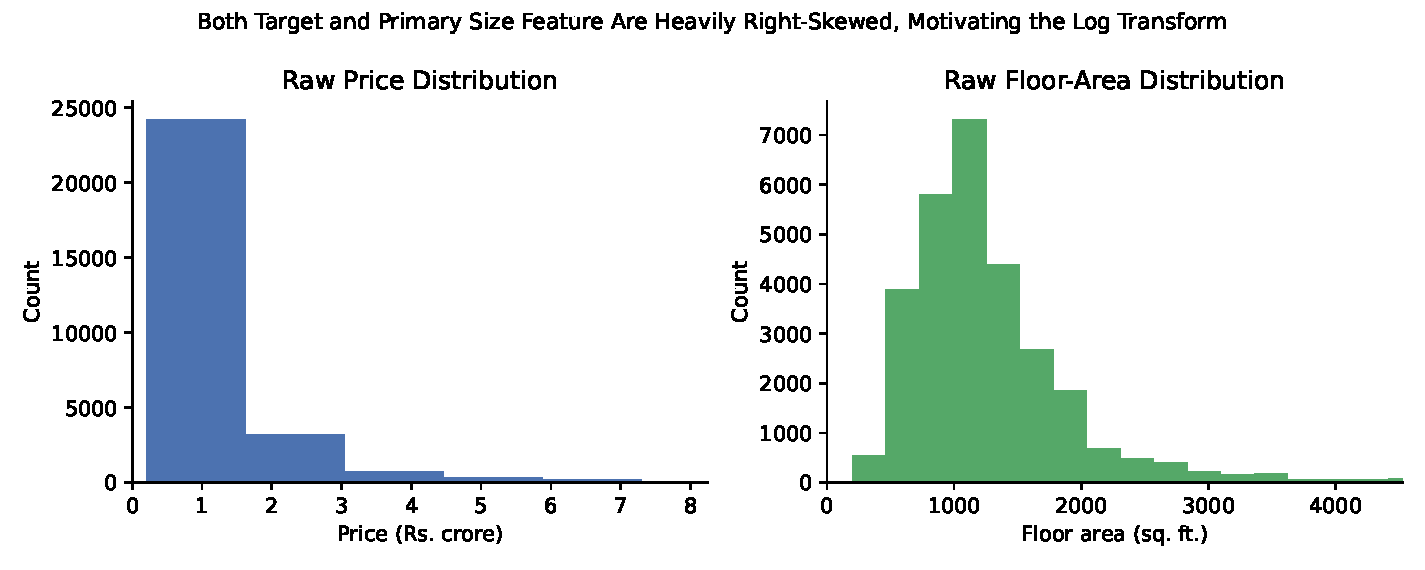
\includegraphics[width=0.85\textwidth]{figures/price_area_distribution.pdf}
\caption{Distribution of raw listing price (in crore rupees) and floor area (in
square feet) before cleaning, six-city combined data. Both distributions are
strongly right-skewed, motivating the log-transform described in
Section~\ref{sec:feateng}.}
\label{fig:distribution}
\end{figure}

\section{Cleaning}
Schema inspection showed that each amenity column uses a placeholder value of 9 to
mean ``not recorded'' for roughly 70\% of rows; every value outside $\{0,1\}$ is
converted to a genuine missing value rather than assumed to be one specific guessed
code. Exact duplicate rows are removed, dropping 3{,}828 of the 32{,}963 rows
(11.6\%) and leaving 29{,}135 rows for modelling. Rows with non-positive price or
area are also dropped as data-entry errors.

\section{Feature Engineering}
\label{sec:feateng}
The free-text locality column has a long tail of names occurring once or twice;
localities occurring fewer than 15 times in the training split are collapsed into an
``other'' category before encoding, and the locality and city columns are then
encoded with scikit-learn's cross-fitted \texttt{TargetEncoder}, fit only on the
training split so no calibration or test information leaks into the encoding. Price
and floor area, both heavily right-skewed (Figure~\ref{fig:distribution}), are
log-transformed. Price-per-area-style features are deliberately excluded, since they
are computed from the target and would produce impressive but meaningless accuracy.
No feature based on caste, religion, or community composition is used, a deliberate
constraint given that locality names in Indian data can otherwise act as a proxy for
such attributes.

\section{Splitting, Training, and Uncertainty}
The cleaned data is split 60/20/20 into training, calibration, and test portions. The
calibration split is used only to build price ranges, never to fit or tune a model;
the test split is touched exactly once, for final evaluation. Three models --
regularised linear regression (Ridge), Random Forest, and XGBoost -- are tuned by
cross-validation on the training split alone (Table~\ref{tab:cv}, Figure~\ref{fig:cv});
XGBoost was selected as the point-prediction model. Price ranges at the 90\% level are
built two ways using MAPIE's current (v1) API: split-conformal on the XGBoost model,
and an adaptive, quantile-based variant (CQR) using a triplet of
\texttt{HistGradientBoosting} quantile models, since MAPIE's CQR implementation does
not currently support XGBoost directly. Both arms are compared against a no-range
baseline and a naive fixed-width band calibrated on the same calibration split, so the
value of an adaptive range is demonstrated rather than assumed.

\begin{figure}[H]
\centering
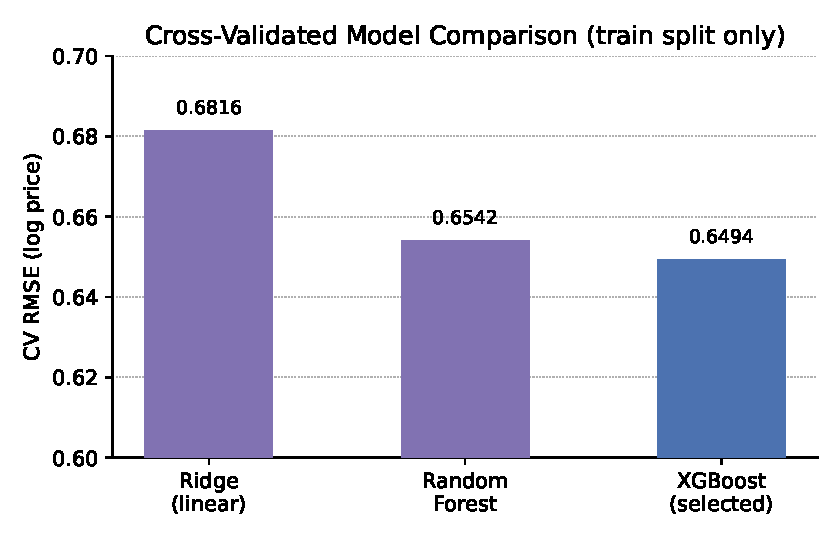
\includegraphics[width=0.7\textwidth]{figures/cv_leaderboard.pdf}
\caption{Cross-validated log-price RMSE for the three candidate models, training
split (lower is better). XGBoost was selected.}
\label{fig:cv}
\end{figure}

\section{Explanation and Confidence}
\label{sec:explconf}
Per-house explanations are produced from XGBoost's native feature-contribution
output rather than the \texttt{shap} package -- the two are mathematically
equivalent for tree ensembles, and avoiding \texttt{shap} keeps the deployed
service's memory footprint well within the 512\,MB budget of its hosting tier. A
confidence flag combines three signals computed on the calibration split: the width
of a house's price range relative to its predicted price, how unusual its features
are relative to the training data (via an Isolation Forest fit on the training split
only), and how many important fields were left unanswered. Each signal's threshold is
its own 90th percentile on the calibration split; a prediction is flagged when at
least two of the three signals fire, or when any single signal is extreme (above its
97th percentile) -- the second rule was added after finding that range width and
novelty are, for this dataset, only weakly correlated, so requiring two ordinary
signals to agree could under-flag genuinely unusual houses that only one signal
catches strongly.

\subsection{Confidence Flag Calibration}
Figure~\ref{fig:novelty} makes this weak correlation concrete: on the calibration
split ($n=5{,}827$), the Pearson correlation between a house's novelty score and its
range-width ratio is $r=-0.65$ -- the two signals are, if anything, mildly
anti-correlated rather than reinforcing one another. A house can therefore be highly
novel relative to the training data while still receiving a comparatively narrow
range (because the underlying quantile models happen to agree on it), or vice versa.
This is precisely why the flagging rule combines three independent signals with a
2-of-3 vote rather than relying on any single one, and why the 97th-percentile
``extreme single signal'' override exists: without it, a house that is extremely
novel but only moderately wide-ranged, or extremely wide-ranged but only moderately
novel, could pass through both ordinary thresholds unflagged.

\begin{figure}[H]
\centering
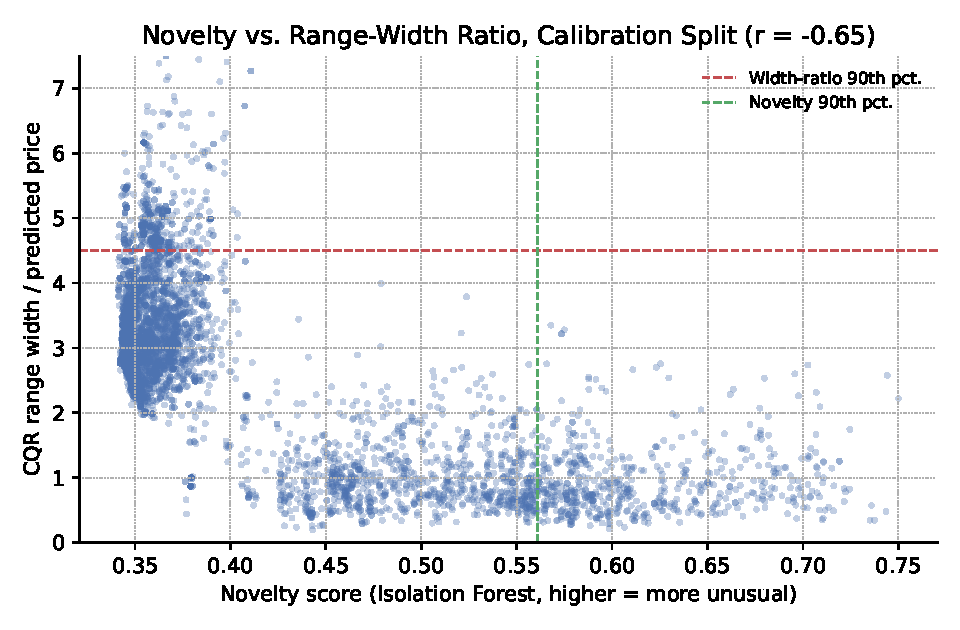
\includegraphics[width=0.75\textwidth]{figures/novelty_vs_width.pdf}
\caption{Novelty score versus range-width ratio on the calibration split
($n=5{,}827$, $r=-0.65$), showing the two signals are not redundant with each
other -- justifying the three-signal, 2-of-3 design described in
Section~\ref{sec:explconf}.}
\label{fig:novelty}
\end{figure}

\section{Deployment}
\subsection{System Architecture}
The trained pipeline is served two ways from the same artefacts (Figure~\ref{fig:arch}):
a FastAPI backend (\texttt{/api/schema}, \texttt{/api/predict}, \texttt{/api/metrics})
behind a hand-built HTML, CSS, and JavaScript frontend, deployed on Render, and a
Streamlit application kept live as a fallback on Streamlit Community Cloud. Both call
the identical trained model, conformal objects, and confidence-flag logic through the
shared \texttt{src/} package -- \texttt{api/inference.py} reuses those modules
directly rather than reimplementing any modelling step, so no ML logic is duplicated
or can silently diverge between the two apps. The FastAPI service loads a trimmed
\texttt{api\_bundle.joblib} that omits the \texttt{shap} package as a runtime
dependency, since XGBoost's native contribution output is used instead
(Section~\ref{sec:explconf}); this matters concretely on Render's free tier, which
caps the service at 512\,MB of memory.

\begin{figure}[H]
\centering
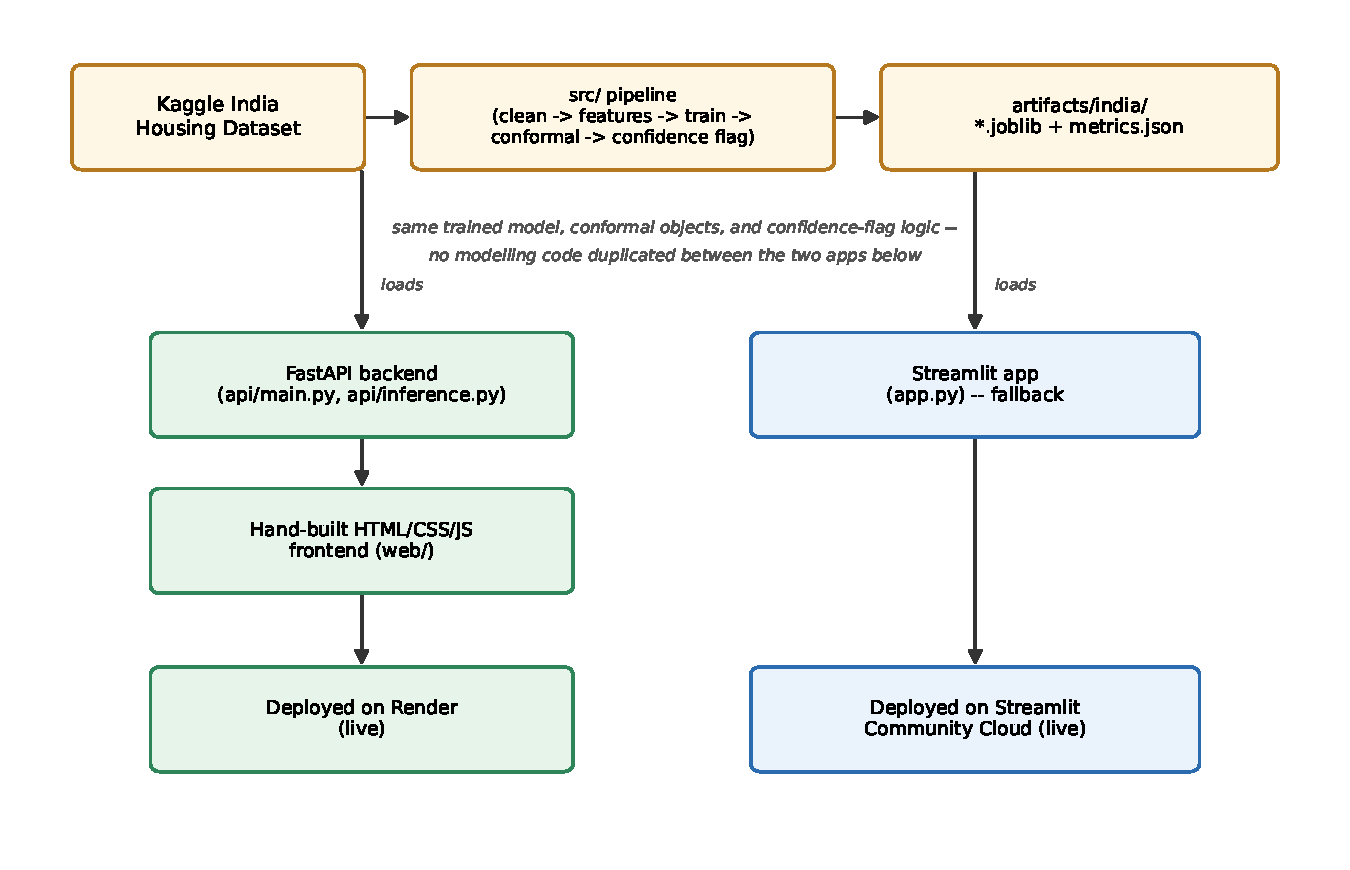
\includegraphics[width=0.95\textwidth]{figures/architecture.pdf}
\caption{System architecture: two frontends served by one shared pipeline, with no
modelling logic duplicated between them.}
\label{fig:arch}
\end{figure}

\subsection{Web Form Design}
The web form treats city and floor area as required, since a price
estimate is least meaningful without either, while locality, bedroom count, and
resale status may be left unanswered, which is tracked by the confidence flag rather
than silently ignored. Figure~\ref{fig:appform} shows the deployed form.

\begin{figure}[H]
\centering
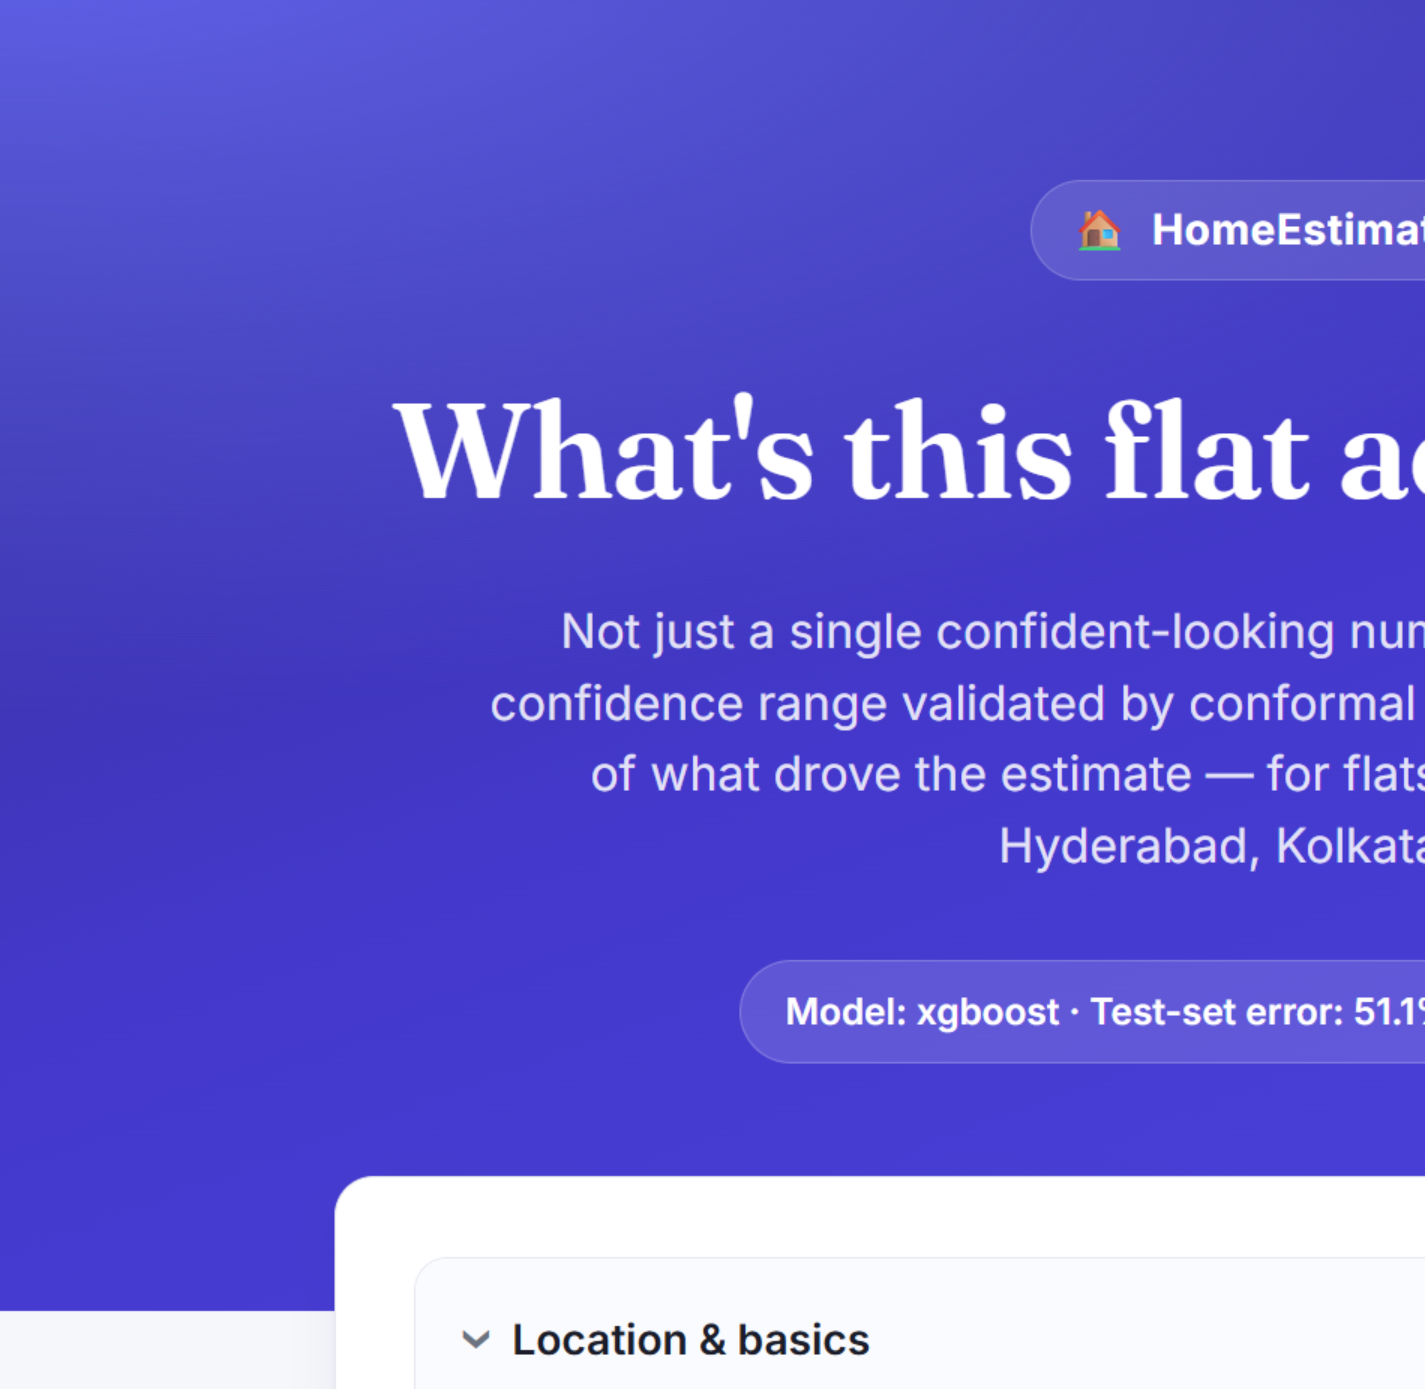
\includegraphics[width=0.8\textwidth]{figures/app_form.png}
\caption{The deployed application's input form (house-price-estimator-india.onrender.com).}
\label{fig:appform}
\end{figure}

% ---------------------------------------------------------------------
% Chapter 4: Results and Analysis
% ---------------------------------------------------------------------
\chapter{Results and Analysis}
\label{ch:results}

All figures in this chapter are computed on the test split, which was touched exactly
once after every modelling and calibration decision was finalised.

\section{Point-Prediction Accuracy}
Table~\ref{tab:cv} shows the cross-validated log-price RMSE used to select XGBoost as
the point-prediction model on the training split. Table~\ref{tab:point} shows its
accuracy on the held-out test split, reported both on the log scale used for model
selection and in currency terms that are directly interpretable.

\begin{table}[h]
\centering
\caption{Cross-validated log-price RMSE on the training split (lower is better).}
\label{tab:cv}
\begin{tabular}{lc}
\toprule
Model & CV RMSE (log price) \\
\midrule
Ridge (linear baseline) & 0.6816 \\
Random Forest & 0.6542 \\
\textbf{XGBoost (selected)} & \textbf{0.6494} \\
\bottomrule
\end{tabular}
\end{table}

\begin{table}[h]
\centering
\caption{Point-prediction accuracy on the test split (XGBoost).}
\label{tab:point}
\begin{tabular}{lc}
\toprule
Metric & Value \\
\midrule
RMSE (log price) & 0.656 \\
Mean Absolute Error & Rs.\,60.21 lakh \\
RMSE & Rs.\,2.02 crore \\
MAPE & 51.1\% \\
\bottomrule
\end{tabular}
\end{table}

A MAPE of 51.1\% is markedly weaker than a well-behaved regression problem, and it is
reported here without averaging it away. It reflects the dataset's own stated
limitations -- asking prices rather than confirmed sales, no transaction date, and
roughly 70\% missing amenity data -- rather than a failure of the modelling approach;
Figure~\ref{fig:bracket} breaks this down further by price bracket.

\section{Price-Range Coverage}
Table~\ref{tab:coverage} and Figure~\ref{fig:coverage} compare all four range-building
methods against their shared 90\% target. Every method lands within about one
percentage point of the target, which is itself a result: it shows the calibration
procedure works, and that the adaptive (CQR) arm achieves the same reliability as the
simpler alternatives while, as shown by its narrower median width, concentrating
its width where it is actually needed rather than applying it uniformly.

\begin{table}[h]
\centering
\caption{90\% price-range coverage and width by method, test split.}
\label{tab:coverage}
\begin{tabular}{lccc}
\toprule
Method & Coverage & Avg. width & Median width \\
\midrule
CQR (adaptive) & 89.9\% & Rs.\,2.35 Cr & Rs.\,2.02 Cr \\
Split-conformal (XGBoost) & 90.5\% & Rs.\,2.19 Cr & Rs.\,1.70 Cr \\
Split-conformal (HistGBR) & 90.3\% & Rs.\,2.10 Cr & Rs.\,1.64 Cr \\
Naive fixed-width baseline & 90.1\% & Rs.\,2.18 Cr & Rs.\,2.18 Cr \\
\bottomrule
\end{tabular}
\end{table}

\begin{figure}[H]
\centering
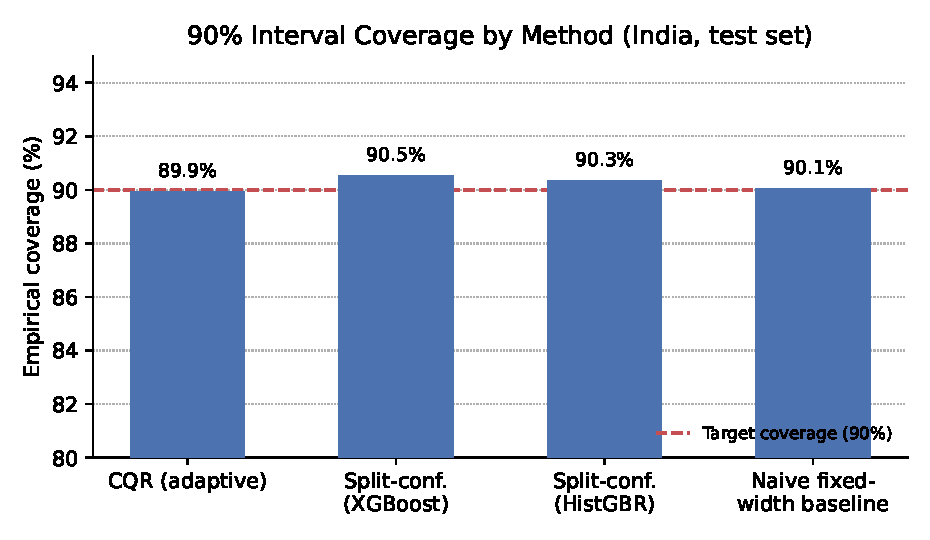
\includegraphics[width=0.72\textwidth]{figures/coverage_by_method.pdf}
\caption{Empirical 90\% coverage achieved by each range-construction method on the
test split, against the 90\% target (dashed line).}
\label{fig:coverage}
\end{figure}

\begin{figure}[H]
\centering
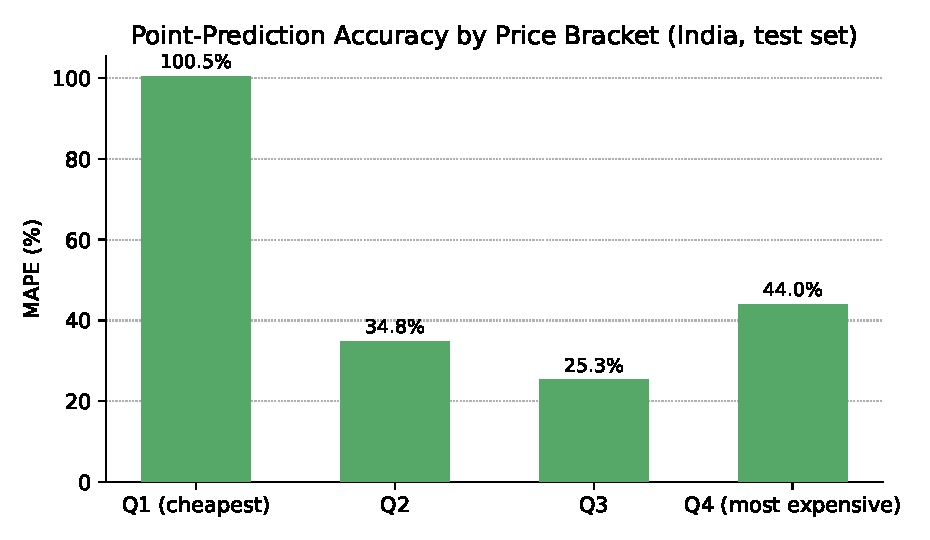
\includegraphics[width=0.72\textwidth]{figures/mape_by_bracket.pdf}
\caption{Point-prediction MAPE by price quartile, test split. The cheapest bracket
(Q1) is proportionally hardest, consistent with asking-price noise mattering more
for lower-value listings.}
\label{fig:bracket}
\end{figure}

\section{Coverage by City}
No city in the test set was excluded from this breakdown, since every one had at
least the minimum 100 test rows required to report a reliable per-segment number
(Table~\ref{tab:city}, Figure~\ref{fig:city}). Coverage stays close to 90\% in every
city, though average range width varies by roughly a factor of three between the
cheapest and most expensive markets, showing that the adaptive range genuinely tracks
each city's own price volatility rather than applying one national-average width
everywhere.

\begin{table}[h]
\centering
\caption{CQR coverage and average width by city, test split (all $n \geq 100$).}
\label{tab:city}
\begin{tabular}{lccc}
\toprule
City & $n$ (test) & Coverage & Avg. width \\
\midrule
Bangalore & 1{,}107 & 91.9\% & Rs.\,2.02 Cr \\
Chennai & 892 & 90.2\% & Rs.\,1.56 Cr \\
Delhi & 842 & 89.0\% & Rs.\,3.31 Cr \\
Hyderabad & 395 & 88.9\% & Rs.\,0.92 Cr \\
Kolkata & 1{,}260 & 89.2\% & Rs.\,1.97 Cr \\
Mumbai & 1{,}331 & 89.7\% & Rs.\,3.33 Cr \\
\bottomrule
\end{tabular}
\end{table}

\begin{figure}[H]
\centering
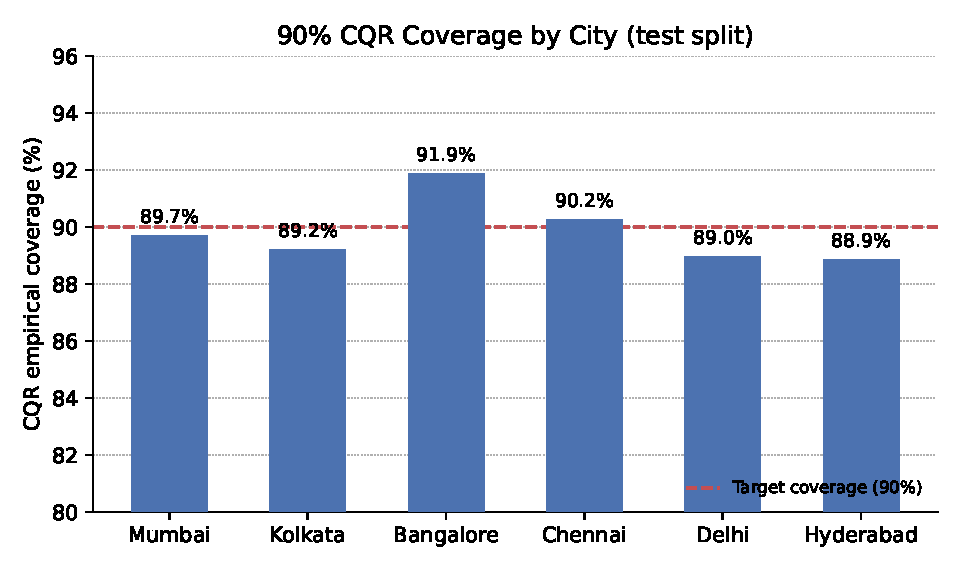
\includegraphics[width=0.75\textwidth]{figures/coverage_by_city.pdf}
\caption{CQR coverage by city, test split, against the 90\% target (dashed line).
All six cities land within roughly two points of target.}
\label{fig:city}
\end{figure}

\section{Does the Confidence Flag Mean Anything}
The confidence flag is only useful if a flagged prediction is actually worse; Table
\ref{tab:flag} confirms this on the test split, which the flag's calibration never
saw. Flagged predictions show 62.1\% MAPE against 50.4\% for the rest -- a real,
sizeable gap, and evidence that the flag is catching genuine weaknesses in the model
rather than adding noise.

\begin{table}[h]
\centering
\caption{Confidence-flag validation, test split.}
\label{tab:flag}
\begin{tabular}{lccc}
\toprule
Group & $n$ & MAE & MAPE \\
\midrule
Flagged low-confidence & 310 & Rs.\,83.64 lakh & 62.1\% \\
Not flagged & 5{,}517 & Rs.\,58.90 lakh & 50.4\% \\
\bottomrule
\end{tabular}
\end{table}

\section{The Deployed Application in Use}
Figure~\ref{fig:appresult} shows a live prediction on the deployed application for a
1,450 sq.\ ft.\ resale flat in Whitefield, Bangalore: a predicted price of Rs.\,73.99
lakh with a 90\% range of Rs.\,27.57 lakh to Rs.\,2.97 crore, rendered with the same
range-visualisation logic evaluated quantitatively in
Section~\ref{sec:feateng}--\ref{ch:results} above. This end-to-end trace, from a raw
form submission through the deployed API back to a rendered chart, is what
Section~\ref{sec:objectives}'s fifth objective -- a working web application, evaluated
honestly -- refers to in practice, not only as a set of offline numbers.

\begin{figure}[H]
\centering
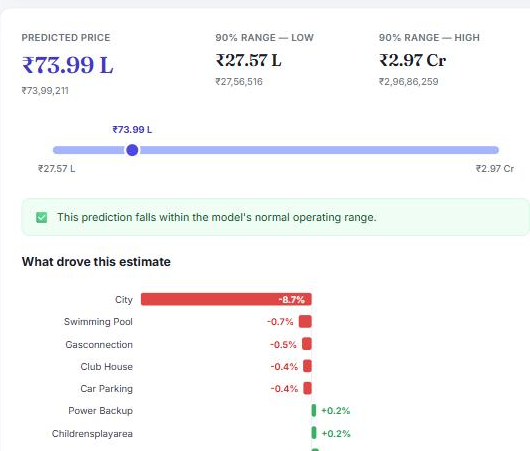
\includegraphics[width=0.68\textwidth]{figures/app_prediction.png}
\caption{A live prediction on the deployed application, showing the predicted price,
the 90\% range, the low-confidence check, and the per-feature explanation chart for
a sample Bangalore flat.}
\label{fig:appresult}
\end{figure}

The application also exposes its own validation numbers directly to the user, rather
than asking them to trust the model blindly: an in-app ``Model performance \&
validation'' panel (Figure~\ref{fig:appmetrics}) surfaces the same point-accuracy and
coverage-by-method figures reported in Tables~\ref{tab:point} and
\ref{tab:coverage}, computed once at deploy time and served directly from
\texttt{/api/metrics} rather than recomputed per request.

\begin{figure}[H]
\centering
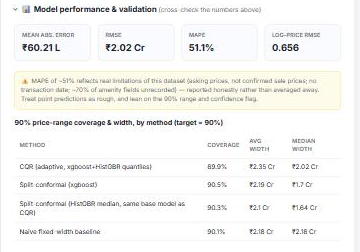
\includegraphics[width=0.88\textwidth]{figures/app_metrics.png}
\caption{The deployed application's ``Model performance \& validation'' panel,
showing the same point-accuracy and coverage-by-method numbers reported in
Tables~\ref{tab:point} and \ref{tab:coverage}, surfaced directly to the user.}
\label{fig:appmetrics}
\end{figure}

% ---------------------------------------------------------------------
% Chapter 5: Conclusion and Future Work
% ---------------------------------------------------------------------
\chapter{Conclusion and Future Work}

All five objectives set out in Section~\ref{sec:objectives} were met on real data, not
only in principle. Three candidate models were cleaned, trained, and compared honestly
rather than only reporting the winner; price ranges were built with conformal
prediction and verified, not assumed, to reach their claimed 90\% coverage on data
touched exactly once; every prediction carries a feature-level explanation and a
confidence flag shown to correlate with real prediction error; and the whole system
runs as a deployed web application rather than a notebook. The project's central
finding is that reliability can be measured and delivered even when point accuracy is
weak: a 51.1\% MAPE, driven by asking-price noise and missing data rather than a
modelling shortfall, still comes with price ranges that hit their 90\% target and a
confidence flag that reliably identifies the predictions least worth trusting.

Table~\ref{tab:traceability} traces each objective from Section~\ref{sec:objectives}
to the chapter and section where it was addressed and verified, so the correspondence
between what was promised and what was delivered is explicit rather than left to be
inferred.

\begin{table}[h]
\centering
\caption{Objectives traceability.}
\label{tab:traceability}
\begin{tabular}{p{0.08\textwidth}p{0.44\textwidth}p{0.38\textwidth}}
\toprule
\# & Objective & Addressed in \\
\midrule
1 & Clean data; train and compare Ridge, Random Forest, XGBoost & Sections~3.1--3.4, 4.1 \\
2 & 90\% conformal price ranges, empirically verified & Sections~3.4, 4.2 \\
3 & Per-house feature explanations & Section~3.5 \\
4 & Low-confidence flag for unusual/wide-range houses & Sections~3.5, 4.4 \\
5 & Working web application, evaluated honestly & Sections~3.6, 4.3, 4.5 \\
\bottomrule
\end{tabular}
\end{table}

The clearest limitation is the data itself. Asking prices are not confirmed sales,
there is no transaction date to track the market over time, and roughly 70\% of
amenity information is unrecorded. None of this can be fixed by a better model; it
requires a better data source. Future work should prioritise, in order: (1) a
verified-transaction dataset with sale dates, which would likely improve point
accuracy far more than further model tuning; (2) extending coverage to more Indian
cities and periodically retraining as prices move, since the current model reflects
only the period its training data was collected in; (3) a native mobile client
against the existing FastAPI backend, which already separates the model-serving API
from the frontend; and (4) revisiting the confidence flag's two-tier design as more
data becomes available, since the anti-correlation found between range width and
novelty for this dataset (Section~\ref{sec:explconf}) is itself worth further
investigation rather than only working around.

% ---------------------------------------------------------------------
% References
% ---------------------------------------------------------------------
\chapter*{References}
\addcontentsline{toc}{chapter}{References}
\begin{enumerate}[label={[\arabic*]}, leftmargin=2.2em]

\item ``Housing Prices in Metropolitan Areas of India,'' Kaggle dataset,
\url{https://www.kaggle.com/datasets/ruchi798/housing-prices-in-metropolitan-areas-of-india}

\item L.\ Grinsztajn, E.\ Oyallon, and G.\ Varoquaux, ``Why Do Tree-Based Models Still
Outperform Deep Learning on Typical Tabular Data?,'' in \emph{Proc.\ NeurIPS Datasets
and Benchmarks Track}, 2022. arXiv:2207.08815.

\item S.\ Rosen, ``Hedonic Prices and Implicit Markets: Product Differentiation in
Pure Competition,'' \emph{Journal of Political Economy}, vol.\ 82, no.\ 1, pp.\
34--55, 1974.

\item Y.\ Romano, E.\ Patterson, and E.\ J.\ Cand\`es, ``Conformalized Quantile
Regression,'' in \emph{Advances in Neural Information Processing Systems}, vol.\ 32,
2019. arXiv:1905.03222.

\item A.\ N.\ Angelopoulos and S.\ Bates, ``A Gentle Introduction to Conformal
Prediction and Distribution-Free Uncertainty Quantification,'' arXiv:2107.07511,
2021.

\item S.\ M.\ Lundberg and S.\ Lee, ``A Unified Approach to Interpreting Model
Predictions,'' in \emph{Advances in Neural Information Processing Systems}, vol.\ 30,
2017. arXiv:1705.07874.

\item T.\ Chen and C.\ Guestrin, ``XGBoost: A Scalable Tree Boosting System,'' in
\emph{Proc.\ ACM SIGKDD}, 2016. arXiv:1603.02754.

\item ``Exploring the Role of AI in the Closure of Zillow Offers,'' \emph{Journal of
Information Systems Education}, vol.\ 35, no.\ 1, pp.\ 67--72, 2024.

\end{enumerate}

% ---------------------------------------------------------------------
% Appendix
% ---------------------------------------------------------------------
\appendix
\chapter{Project Directory Structure}

The repository is organised so that no modelling logic is duplicated between the two
deployed applications; both call directly into \texttt{src/}.

{\scriptsize
\begin{verbatim}
src/
|-- config.py                  # paths, seed, per-market registry
|-- data/                      # acquire, clean, split
|-- features/                  # per-market feature engineering + shared preprocessing
|-- models/                    # train/tune, quantile models, persistence
|-- uncertainty/               # conformal prediction (MAPIE) + baselines
|-- explain/
|   |-- feature_names.py       # shap-independent column-name aggregation (shared)
|   `-- shap_explainer.py      # SHAP explanations (pipeline/Streamlit only)
|-- confidence/                # low-confidence flag
|-- evaluation/                # metrics, coverage/width tables, report writer
`-- pipeline.py                # end-to-end orchestration
api/
|-- main.py                    # FastAPI app: /api/schema, /api/predict, /api/metrics
`-- inference.py                # request handling, reuses src/ (no ML logic duplicated)
web/                            # static HTML/CSS/JS frontend served by api/main.py
app.py                          # Streamlit app (kept live as a fallback)
tests/                          # unit tests
reports/                        # generated evaluation reports
artifacts/{ames,india}/         # model_bundle.joblib (full) + api_bundle.joblib (trimmed)
render.yaml                     # Render.com Blueprint for the FastAPI service
requirements-api.txt            # slim deps for the deployed API (no shap/streamlit/kaggle)
\end{verbatim}
}

\end{document}
